%!TEX root = main.tex

Let us begin by reviewing the concept of \emph{constrained optimization}, and some associated notation and terminology.  The objective is the search for extrema of a function $f \colon D \to \field{R}$ where the input values $\x$ belong in an open subset $D \subseteq \field{R}^d$ and satisfy a finite set of \emph{constraints} of the form
\begin{gather*}
g_1(\x) \leq 0, g_2(\x) \leq 0, \dotsc, g_m(\x) \leq 0, \\
h_1(\x) = 0, h_2(\x) = 0, \dotsc, h_\ell(\x) = 0,
\end{gather*}
for real-valued functions $g_k\colon \field{R}^d \to \field{R}, (1\leq k \leq m)$, $h_k \colon \field{R}^d \to \field{R}, (1\leq k \leq \ell)$.
\index{Constrained optimization}
\index{Constraint}

For simplicity, we write instead
\begin{equation}\label{equation:programP}
(P) \begin{cases} \min_{x\in D}f(\x) \\ g_1(\x) \leq 0, \dotsc, g_m(\x) \leq 0 \\ h_1(\x) = 0, \dotsc, h_\ell(\x) =0 \end{cases}
\end{equation}
or better, if we set 
\begin{equation*}
S = \{ \x \in D : g_1(\x) \leq 0, \dotsc, g_m(\x) \leq 0, h_1(\x) = 0, \dotsc, h_\ell(\x)=0\},
\end{equation*} we may simply write 
\begin{equation*}
(P) = \min_{x\in S} f.
\end{equation*}
We refer to it as the \emph{program} $(P)$.\index{Program} The function $f$ is called the \emph{objective function of }$(P)$\index{Objective function of $(P)$}.  We refer to the functions $g_k$ as the \emph{inequality constraints}.  The functions $h_k$ are called the \emph{equality constraints}.\index{Constraint!inequality}\index{Constraint!equality}

A point $\x \in D$ that satisfies all the constraints of the program $(P)$ is said to be \emph{feasible}.\index{Feasible!point}  The set of all feasible points is called the \emph{feasibility region} of $(P)$.\index{Feasibility region}  If the feasibility region is non-empty, we say that the program $(P)$ is \emph{consistent}\index{Program!consistent}. If a feasible point satisfies $g_k(\x) < 0$ for all inequality constraints, we call it a \emph{Slater point}\index{Slater point}. Consistent programs $(P)$ that have Slater points are said to be \emph{super-consistent}.
\index{Program!super-consistent}

If the objective function $f$ and all constraints $g_k$, $h_k$ of a program $(P)$ are linear functions, we denote it by $(LP)$ and refer to it as a \emph{linear program}.  If the objective function, all constraints $g_k$, $h_k$ and the set $D$ are convex, we call $(P)$ a \emph{convex program}.
\index{Program!linear}\index{Program!convex}

\begin{example}\label{example:feasibleP1}
Let $f(x,y)=x^4+y^4$, and consider the program $(P) = \min_{x\in S} f(x,y)$, where $S = \{ (x,y) \in \field{R}^2: x^2 \leq 1, y^2 \leq 1, e^{x+y}\leq 1\}$.

The inequality constraints are $g_1(x,y)=x^2-1$, $g_2(x,y)=y^2-1$ and $g_3(x,y)=e^{x+y}-1\leq 0$ (although you may choose simpler equivalent expressions).  The feasibility region is thus a triangular region (see Figure \ref{figure:feasibleP1}):
\begin{equation*}
S = \{ (x,y) \in \field{R}^2 : \abs{x} \leq 1, \abs{y} \leq 1, x+y \leq 0 \} \neq \emptyset.
\end{equation*}
\begin{figure}[ht!]
\begin{tabular}{cc}
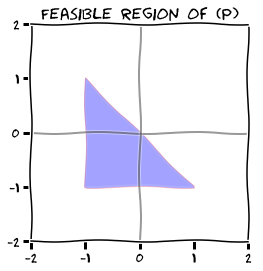
\includegraphics[width=0.5\linewidth]{images/feasibleP1.png} &
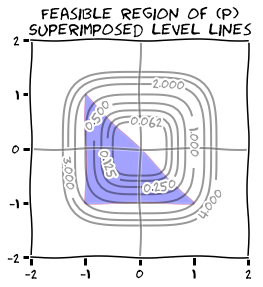
\includegraphics[width=0.5\linewidth]{images/feasibleP2.png} 
\end{tabular}
\caption{Can you tell what are the global maximum and minimum values of $f$ in $S$?}
\label{figure:feasibleP1}
\end{figure}
This is a super-consistent convex program, since any interior point of the triangle $S$ is a Slater point for $(P)$, and all relevant functions are convex.
\end{example}

\begin{definition}
\index{Indices of the binding inequality constraints}
\index{Cone!of improving directions}
\index{Cone!of inward pointing directions for the binding constraints}
\index{Set of tangent directions for equality constraints}
Given a consistent program $(P)$ as defined in \eqref{equation:programP}, for each feasible point $\x \in S$, we define:
\begin{enumerate}
	\item The \emph{cone of improving directions} of $f$ at $\x$, as
	\begin{equation*}
	\mathcal{F}_0(\x) = \{ \v \in \field{R}^d : \norm{\v}=1, \langle \gradient{f}(\x), \v \rangle < 0 \}
	\end{equation*}
	\item The set of \emph{indices of the binding inequality constraints} for $\x$, as
	\begin{equation*}
	\mathcal{I}(\x) = \big\{ k \in \{1, \dotsc, m\} : g_k(\x) = 0 \big\}.
	\end{equation*}
	\item The \emph{cone of inward pointing directions for the binding constraints} at $\x$, as
	\begin{equation*}
	\mathcal{G}_0(\x) = \{ \v \in \field{R}^d : \norm{\v}=1, \langle \gradient{g_k}(\x), \v \rangle < 0 \text{ for all } k \in \mathcal{I}(\x) \}
	\end{equation*}
	\item The set of \emph{tangent directions for the equality constraints} at $\x$, as
	\begin{equation*}
	\mathcal{H}_0(\x) = \{ \v \in \field{R}^d : \langle \gradient{h_k}(\x), \v \rangle = 0, 1 \leq k \leq \ell \}
	\end{equation*}
\end{enumerate}
\end{definition}

\begin{example}
For the program $(P)$ in Example \ref{example:feasibleP1}, consider the feasible points $(0,0)$, $(-1,-1)$ and $(0,-1/2)$.  Since $\gradient{f}(x,y) = [ 4x^3, 4y^3 ]$, we have the following cones on improving direction 
\begin{align*}
\mathcal{F}_0(0,0) &= \emptyset, \\
\mathcal{F}_0(-1,-1) &= \{ \v = (v_1, v_2) \in \field{R}^2 : \norm{\v}=1, v_1+v_2 > 0 \}, \\
\mathcal{F}_0(0,-1/2) &= \{ \v = (v_1, v_2) \in \field{R}^2 : \norm{\v} = 1, v_2 > 0 \}
\end{align*}
The indices of binding inequality constraints are
\begin{equation*}
\mathcal{I}(0,0) = \{ 3 \}, \quad \mathcal{I}(-1,-1) = \{ 1,2 \}, \quad \mathcal{I}(0,-1/2)= \emptyset,
\end{equation*}
and therefore, the cones of inward pointing directions for the binding constraints are
\begin{align*}
\mathcal{G}_0(0,0) &= \{ \v = (v_1, v_2) \in \field{R}^2 : \norm{\v}=1, v_1+v_2 < 0 \}, \\
\mathcal{G}_0(-1,-1) &= \{ \v = (v_1, v_2) \in \field{R}^2 : \norm{\v}=1, v_1 > 0,  v_2 > 0 \},\\
\mathcal{G}_0(0,-1/2) &= \emptyset.
\end{align*}
Since there are no equality constraints, we do not have any sets of tangent directions.

\begin{figure}[ht!]
\begin{tabular}{cc}
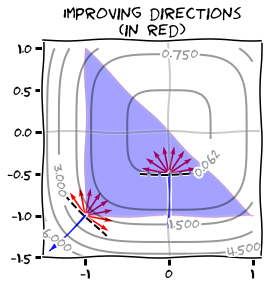
\includegraphics[width=0.5\linewidth]{images/improvingdirections.png} &
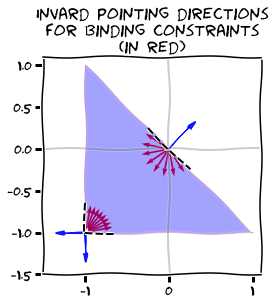
\includegraphics[width=0.5\linewidth]{images/inwarddirections.png} 
\end{tabular}
\caption{Cones for $(0,0)$, $(-1,-1)$ and $(0,-1/2)$.}
\label{figure:cones}
\end{figure}
\end{example}

\separator 

In the following sections we are going to discuss necessary and sufficient conditions for the existence of (strict) global minima for any consistent program $(P)$.  We are going to focus exclusively on the main results without showing their proofs (if interested in those proofs, consult \cite[lec6\_constr\_opt]{Freund2004nonlinear}).\index{Minimum!global}\index{Minimum!strict global}\index{Minimum!local}\index{Minimum!strict local}

\section{Necessary Conditions}
We begin with two results that focus on the structure of the equality constraints.
\begin{theorem}[Geometric Necessary Condition for Linear Equality Constraints]\index{Theorem!Geometric necessary condition}
If $(P)$ is a consistent program with linear equality constraints $h_k(\x) = \langle \boldsymbol{a}_k, \x \rangle + b_k$ ($\boldsymbol{a}_k \in \field{R}^d$, $b_k \in \field{R}$) for all $1 \leq k \leq \ell$, then for all feasible local minima $\x \in S$,
\begin{equation*}
\mathcal{F}_0(\x) \cap \mathcal{G}_0(\x) \cap \mathcal{H}_0(\x) = \emptyset.
\end{equation*}
\end{theorem}

\begin{theorem}[Geometric Necessary Condition for Linearly Independent Equality Constraints]\index{Theorem!Geometric necessary condition}
If $\x \in S$ is a feasible local minimum for the consistent program $(P)$, and the gradient vectors $\{ \gradient{h_k}(\x) : 1 \leq k \leq \ell \}$ are linearly independent, then $\mathcal{F}_0(\x) \cap \mathcal{G}_0(\x) \cap \mathcal{H}_0(\x) = \emptyset$.
\end{theorem}

\separator

As a consequence, an algebraic version of this geometric necessary condition gives the following result.

\begin{theorem}[Fritz John Necessary Conditions]\index{Theorem!Fritz John necessary conditions}\label{theorem:FritzJohn}
If $\x \in S$ is a feasible local minimum of the consistent program $(P)$, then there exist $\lambda_k \geq 0$ for $0\leq k \leq m$, and $\mu_1, \dots, \mu_\ell \in \field{R}$ so that
\begin{enumerate}
 	\item $[\lambda_0, \lambda_1, \dotsc, \lambda_m, \mu_1 \dotsc, \mu_\ell ] \neq \boldsymbol{0}$,
 	\item $\lambda_k g_k(\x) = 0$ for all $1 \leq k \leq m$.
 	\item $\lambda_0 \gradient{f}(\x) + \sum_{k=1}^m \lambda_k \gradient{g_k}(\x) + \sum_{k=1}^\ell \mu_k \gradient{h_k}(\x) = 0$.
 \end{enumerate}
\end{theorem}

\begin{example}
Continuing with example \ref{example:feasibleP1}, let's check if the point $(0,0)$ is a candidate to optimal solution of this program.  Let's use Theorem \ref{theorem:FritzJohn} to verify this claim:
\begin{align*}
\gradient{f}(x,y) &= [ 4x^3, 4y^3 ] &\gradient{f}(0,0) &= [0,0], \\
\gradient{g_1}(x,y) &= [ 2x, 0 ] &\gradient{g_1}(0,0) &= [0,0], \\
\gradient{g_2}(x,y) &= [0, 2y] &\gradient{g_2}(0,0) &= [0,0], \\
\gradient{g_3}(x,y) &= \big[e^{x+y}, e^{x+y} \big] &\gradient{g_3}(0,0) &= [1,1].
\end{align*}
Notice how the gradients \emph{line up} nicely---can we find $\lambda_k \geq 0$ so that:
\begin{enumerate}
	\item $[\lambda_0, \lambda_1, \lambda_2, \lambda_3] \neq [0,0,0,0]$,
	\item $\lambda_1=\lambda_2=0$ (since $\lambda_1 g_1(0,0) = -2\lambda_1$ and $\lambda_2 g_2(0,0) = -2\lambda_2$), and
	\item the following linear combination is equal to $[0,0]$
	\begin{gather*}
	\lambda_0\gradient{f}(0,0) + \lambda_1 \gradient{g_1}(0,0) + \lambda_2 \gradient{g_2}(0,0) + \lambda_3 \gradient{g_3}(0,0) = [0,0], \\
	\lambda_0[0,0] + \lambda_1[0,0] + \lambda_2[0,0] + \lambda_3[1,1] = [0,0],
	\end{gather*}
\end{enumerate}
We may select, for instance $\lambda_0=1$, $\lambda_1=\lambda_2=\lambda_3=0$, which proves that the point $(0,0)$ is indeed a candidate for optimal solution of $(P)$.
\end{example}

\separator
Further properties of the involved functions provide us with simpler sets of conditions

\begin{theorem}[Karush-Kuhn-Tucker Necessary Conditions]\index{Theorem!Karush-Kuhn-Tucker}\index{Theorem!KKT necessary conditions}\label{theorem:KKTnecessary}
If $\x \in S$ is a feasible local minimum of the consistent program $(P)$ for which all the vectors $\{ \gradient{h_k}(\x), \gradient{g_j}(\x) : 1 \leq k \leq \ell, j \in \mathcal{I}(\x) \}$ are linearly independent, then there exist $\lambda_k \geq 0$ for $1\leq k \leq m$, and $\mu_1, \dots, \mu_\ell \in \field{R}$ so that
\begin{enumerate}
 	\item\label{item:KKTnecessary1} $\lambda_k g_k(\x) = 0$ for all $1 \leq k \leq m$.
 	\item\label{item:KKTnecessary2} $\gradient{f}(\x) + \sum_{k=1}^m \lambda_k \gradient{g_k}(\x) + \sum_{k=1}^\ell \mu_k \gradient{h_k}(\x) = 0$.
 \end{enumerate}
\end{theorem}

\begin{remark}\index{Karush-Kuhn-Tucker!conditions}\index{Karush-Kuhn-Tucker!multipliers}
The conditions \ref{item:KKTnecessary1} and \ref{item:KKTnecessary2} of Theorem \ref{theorem:KKTnecessary} are called \emph{the KKT conditions} of the program $(P)$ in the literature.   The values $\lambda_k$, $\mu_k$ are called \emph{multipliers}.
\end{remark}

\begin{example}\label{example:feasibleP3}
Set $f(x,y)=(x-12)^2+(y+6)^2$.  Consider the program $(P)$ designed to find the global minimum of this function on the set $S=\{ (x,y) \in \field{R}^2 : x^2+3x+y^2-4.5y \leq 6.5, (x-9)^2 +y^2 \leq 64, 8x+4y=20 \}$.  We want to prove that the point $(2,1)$ is a good candidate for optimal solution of $(P)$.
The point $(2,1)$ is feasible.  To see this, set 
\begin{align*}
g_1(x,y) &=x^2+3x+y^2-4.5y-6.5, \\
g_2(x,y) &=(x-9)^2+y^2-64, \\
h_1(x,y) &=8x+4y-20,
\end{align*}
(or simpler equivalent constraints), and notice that
\begin{equation*}
g_1(2,1)=0, \quad g_2(2,1)=-14, \quad h_1(2,1)=0.
\end{equation*}
\begin{figure}[ht!]
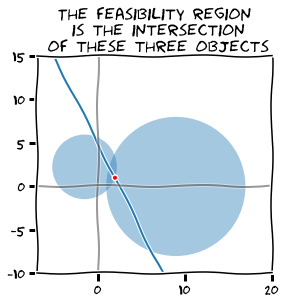
\includegraphics[width=0.5\linewidth]{images/feasibleP3.png}
% \begin{python}
% import numpy as np, matplotlib.pyplot as plt
% # plt.xkcd();
% from matplotlib.patches import Circle
% from matplotlib.collections import PatchCollection

% fig, ax = plt.subplots()
% ax.set_aspect('equal')
% patches = [Circle((-3/2,9/4), np.sqrt(221/16)), Circle((9,0), 8)]
% p = PatchCollection(patches, alpha=0.4)
% ax.add_collection(p)
% plt.xlim(-7,20)
% plt.ylim(-10,15)
% plt.plot([-5,20],[15,-35])
% plt.plot(2,1,'r.')
% plt.plot([0,0],[-10,15],'k',alpha=0.4)
% plt.plot([-7,20],[0,0],'k', alpha=0.4)
% plt.title("The feasibility region\n is the intersection\n of these three objects")
% plt.show()
% \end{python}
\caption{Feasibility region for $(P)$ in example \ref{example:feasibleP3}}
\label{figure:feasibleP3}
\end{figure}
We have concluded that $(P)$ is consistent.  Notice that, $\mathcal{I}(2,1) = \{ 1 \}$, since $g_1(2,1) = 0$, $g_2(2,1) \neq 0$.  Further,
\begin{align*}
\gradient{f}(x,y)   &= [ 2(x-12), 2(y+6) ] &\gradient{f}(2,1)   &= [-20, 14], \\
\gradient{g_1}(x,y) &= [ 2x+3, 2y-4.5 ]    &\gradient{g_1}(2,1) &= [  7, -2.5], \\
\gradient{g_2}(x,y) &= [ 2(x-9), 2y ]      &\gradient{g_2}(2,1) &= [-14, 2], \\
\gradient{h_1}(x,y) &= [ 8, 4]             &\gradient{h_1}(2,1) &= [  8, 4], 
\end{align*}
The vectors $\gradient{g_1}(2,1) = [7,-2.5]$ and $\gradient{h_1}(2,1)=[8,4]$ are linearly independent.  Therefore, to verify that $(2,1)$ is candidate for optimal solution of $(P)$, we may now use Theorem \ref{theorem:KKTnecessary}.  The KKT conditions read as follows: we are looking for $\lambda_k \geq 0, \mu_1 \in \field{R}$ so that $\lambda_k g_k(2,1)=0$ ($k=1,2$) and
\begin{equation*}
\gradient{f}(2,1) + \lambda_1 \gradient{g_1}(2,1) + \lambda_2 \gradient{g_2}(2,1) + \mu_1 \gradient{h_1}(2,1) = [0,0], 
\end{equation*}
Let's address the first condition: Since $g_1(2,1)=0$ and $g_2(2,1)=-14<0$, it must be $\lambda_2=0$.  The second condition turns then into the equation
\begin{equation*}
[-20,14] + \lambda_1 [7,-2.5] + 0 \cdot [-14,2] + \mu_1 [8,4] = [0,0]
\end{equation*}
or equivalently
\begin{equation*}
\begin{bmatrix} 7 & 8 \\ -2.5 & 4 \end{bmatrix} \begin{bmatrix} \lambda_1 \\ \mu_1 \end{bmatrix} = \begin{bmatrix} 20 \\ -14 \end{bmatrix},
\end{equation*}
which gives $\lambda_1=4$, and $\mu_1=-1$.  This proves that the point $(2,1)$ is indeed a good candidate for the optimal solution of $(P)$.
\end{example}

\separator

There are other instances in which the KKT conditions can be used instead of those in the Fritz John Theorem.

\begin{theorem}[Slater Necessary Condition]\label{theorem:Slater}\index{Theorem!Slater condition}
Suppose that the inequality constraints $g_k$ of a super-consistent program $(P)$ are pseudo-convex ($1\leq k \leq m$), the equality constraints $h_k$ are linear ($1\leq k \leq \ell$), and the vectors $\gradient{h_k}(\x)$ are linearly independent at a feasible point $\x$.  Then the KKT conditions \ref{item:KKTnecessary1} and \ref{item:KKTnecessary2} of Theorem \ref{theorem:KKTnecessary} are necessary to characterize $\x$ as an optimal solution of $(P)$.
\end{theorem}

\begin{theorem}\label{theorem:KKTAllLinear}
If all constraints of a consistent program $(P)$ are linear, then the KKT conditions \ref{item:KKTnecessary1} and \ref{item:KKTnecessary2} of Theorem \ref{theorem:KKTnecessary} are necessary to characterize optimal solutions of $(P)$.
\end{theorem}

\section{Sufficient Conditions}

It all boils down to a single result.

\begin{theorem}[KKT Sufficient Conditions]\label{theorem:KKTsufficient}\index{Theorem!KKT sufficient conditions}\index{Theorem!Karush-Kuhn-Tucker}
Let $\x \in S$ be a feasible point of the consistent program $(P)$ for which there are multipliers $\lambda_k \geq 0$ ($1\leq k \leq m)$ and $\mu_k \in \field{R}$ ($1\leq k \leq \ell$) satisfying the conditions \ref{item:KKTnecessary1} and \ref{item:KKTnecessary2} of Theorem \ref{theorem:KKTnecessary}. If $f$ is pseudo-convex, $g_k$ is quasi-convex for all $1\leq k \leq m$, and $h_k$ is linear for all $1\leq k \leq \ell$, then $\x$ is a global optimal solution of $(P)$.
\end{theorem}

\begin{example}
We saw that the point $(0,0)$ satisfies the KKT conditions for the super-consistent convex program $(P)$ in Example \ref{example:feasibleP1}.  As a consequence of Theorems \ref{theorem:FritzJohn} and \ref{theorem:KKTsufficient}, this point must be the optimal global minimum of $(P)$.

We also saw that the point $(2,1)$ satisfies the KKT conditions for the program $(P)$ in Example \ref{example:feasibleP3}.  It is not hard to see that this program is super-consistent, $f$ is pseudo-convex, $g_1$ and $g_2$ are quasi-convex, and $h_1$ is linear.  By virtue of Theorems \ref{theorem:KKTnecessary} and \ref{theorem:KKTsufficient}, the point $(2,1)$ must be the optimal solution of $(P)$.
\end{example}

\section*{Key Examples}
In the following section we are going to use the KKT conditions to address the characterization of optimal solutions of generic programs. 

\begin{example}
Let $\boldsymbol{Q}$ be a symmetric $d \times d$ square matrix.  Consider the associated quadratic form $\quadratic{Q}(\x)$.  We wish to find the global \emph{maximum} over all points of this function in the unit ball $\field{B}_d = \{ \x \in \field{R}^d : \norm{\x} \leq 1 \}$.

An equivalent program $(P)$ is thus defined with $f(\x) = -\quadratic{Q}(\x)$ as its objective function, and a single inequality constraint $g_1(\x) = \norm{\x}^2-1$. This is trivially a super-consistent program with a convex inequality constraint.  Checking the KKT conditions to look for the optimal solution is thus justified under the hypothesis of Theorem \ref{theorem:Slater}.  Notice that
\begin{align*}
\transpose{\gradient{f}(\x)} &= -2 \boldsymbol{Q} \transpose{\x}, \\
\gradient{g_1}(\x) &= 2\x;
\end{align*}
therefore, the KKT conditions request the search for $\x \in \field{B}_d$ and $\lambda \geq 0$ so that $\lambda \big(1-\norm{\x}^2 \big)=0$ and $-2\boldsymbol{Q} \transpose{\x} + 2\lambda\transpose{\x} = \transpose{\boldsymbol{0}}$.  

It must be $\norm{\x}=1$ by the first condition.  The second condition states that $\x$ must be an eigenvector of $\boldsymbol{Q}$ with eigenvalue $\lambda$: $\boldsymbol{Q} \transpose{\x} = \lambda \transpose{\x}$.  The value of the objective function in this case is $f(\x) = -\quadratic{Q}(\x) = -\x \boldsymbol{Q} \transpose{\x} = -\lambda \norm{\x}^2= -\lambda$.  In order to obtain the requested global minimum value (different than zero), $\lambda$ has to be the largest non-negative eigenvalue of $\boldsymbol{Q}$, and $\x$ its corresponding normalized eigenvector.
\end{example}

\begin{example}
A simple case of the previous example: Set $\boldsymbol{Q} = \big[ \begin{smallmatrix} 1 & 3 \\ 3 & 1 \end{smallmatrix}\big]$.  The eigenvalues of $\boldsymbol{Q}$ are $-2$ and $4$, and therefore the maximum of the associated quadratic form $\quadratic{Q}(x,y) = x^2+y^2+6xy$ over the ball $x^2+y^2\leq 1$ happens at the (normalized) solution of the system
\begin{equation*}
\begin{bmatrix} 1 & 3 \\ 3 & 1 \end{bmatrix} \begin{bmatrix} x \\ y \end{bmatrix} = 4\begin{bmatrix} x \\ y \end{bmatrix}.
\end{equation*}
This gives the points $\pm(\sqrt{2}/2, \sqrt{2}/2)$.
\end{example}

\begin{example}
Let $\x_0 \in \field{R}^d\setminus\{\boldsymbol{0}\}$ and $r>0$.  Find the point on the sphere of radius $r$, $\field{S}_d=\{ \x \in \field{R}^d: \norm{\x}=r \}$ that is closer to $\x_0$. 

We may write a super-consistent convex program to solve this optimization problem by using $f(\x)=\norm{\x-\x_0}^2$ as objective function, and one equality constraint $h_1(\x)=\norm{\x}^2-r^2$.  With this choice, we are well within the hypothesis of Theorems \ref{theorem:KKTnecessary} and \ref{theorem:KKTsufficient}.  The KKT conditions request $\mu \in \field{R}$ and a point $\x \in \field{R}^d$ with $\norm{\x} = r$ so that
\begin{equation*} 
\gradient{f}(\x) + \mu\gradient{h_1}(\x) = \boldsymbol{0},
\end{equation*}
This gives $2(\x-\x_0)+2\mu\x = \boldsymbol{0}$, or equivalently, $(1+\mu)\x = \x_0$.

It must be $\mu = -1+\norm{\x_0}/r$.  We have then two cases:
\begin{enumerate}
	\item If $\norm{\x_0}=r$, then $\mu=0$ and $\x=\x_0$ is the only solution.
	\item If $\norm{\x_0} \neq r$ (the point $\x_0$ is not on the sphere), then $\x = r\x_0/\norm{\x_0}$.
\end{enumerate}
\end{example}

\begin{example}\index{Linear map}
Find the minimum value of a (real-valued) linear map over the unit ball.

Given $\boldsymbol{a} \in \field{R}^d\setminus\{ \boldsymbol{0}\}$, consider the corresponding linear map $\boldsymbol{L}(\x) = \langle \boldsymbol{a}, \x \rangle$.  We wish to find the minimum value of $\boldsymbol{L}$ over all points in the unit ball $\field{B}_d = \{ \x \in \field{R}^d : \norm{\x} \leq 1 \}$.

An equivalent program $(P)$ is defined with $\boldsymbol{L}$ as its objective function and $g_1(\x) = \norm{\x}^2-1$. This is a super-consistent convex program.  Checking the KKT conditions is justified under the hypothesis of Theorem \ref{theorem:KKTnecessary}. Notice that
\begin{align*}
\gradient{\boldsymbol{L}}(\x) &= \boldsymbol{a}, \\
\gradient{g_1}(\x) &= 2\x;
\end{align*}
therefore, the KKT conditions request the search for $\x \in \field{B}_d$ and $\lambda \geq 0$ so that $\lambda \big( \norm{\x}^2-1 \big)=0$ and $\boldsymbol{a}+2\lambda\x=\boldsymbol{0}$.

This first condition imposes $\norm{\x}=1$.  The second condition requires $\x = -\boldsymbol{a}/(2\lambda)$.  These two put together imply that it must be $\lambda = -\norm{\boldsymbol{a}}/2$, and hence $\x = -\boldsymbol{a}/\norm{\boldsymbol{a}}$.
\end{example}
